\newpage
	\section*{Задание  «Написание скриптов. Циклы»}
	\paragraph*{ 1. Изучить и предоставить краткий теоретический материал по 				использованию аргументов и циклов. \\ \\}

Oболочка bash поддерживает циклы \textit{for, while,}  а также условия \textit{if и case} .\\ 
	
Аргумент цикла \textit{for} может принимать последовательно заданные значения, список файлов, директории, значения из файла (с использованием команд прочтения), таже это могут быть не только простые(однословные) значения, но также и целые фразы. Если на вход подаётся файл, то разделением выступают знаки табуляции, пробелы и переносы строк, чтобы выбрать например по знаку ':', следует записать следующую команду \textit{IFS=:} .\\

Цикл \textit{while} принимает на сравнение значение переменной или выполнение команды. И в \textit{for} и в \textit{while} можно использовать команды \textit{break} и \textit{continue}. Есть возможность использовать вложенные циклы. Также после выполнения цикла переменная хранит последние значение, и с ней можно работать дальше.  \\

В условие \textit{if} подается команда (выполение команды = 0 = переход по then; невыполнение=1=переход по else) или сравнение. Сравнение осуществляется либо численными значениями, либо строками (по кодировке ASCII) условия сравнения строк заключаются в квадратные скобки, чисел в круглые. \\

	\paragraph*{2. Напишите скрипт на bash, который будет определять, в какую возрастную группу попадают пользователи. \\ \\}
	
При запуске скрипт должен вывести сообщение "Enter your name:" и ждать от пользователя ввода имени (команда read). Затем должно быть выведено имя (Например: «The name you entered is <Имя>. Hi <Имя>!»). После чего у пользователя должен быть выбор, продолжать работу или нет. Когда имя введено и сделан выбор, то скрипт должен написать "Enter your age:" и ждать ввода возраста. Когда возраст введен, скрипт пишет на экран "<Имя>, your group is <группа>", где <группа> определяется на основе возраста по следующим правилам: \\

младше либо равно 16: "child", \\

от 17 до 25 (включительно): "youth", \\

старше 25: "adult". \\

После этого скрипт опять выводит сообщение "Enter your name:" и всё начинается по новой. Если в какой-то момент работы скрипта будет введено пустое имя или возраст 0 (недопустимые символы, буквы итп.), то скрипт должен написать на экран "bye" и закончить свою работу. 
	
	\vspace{1cm}	
	
Был выбран следующий алгоритм работы: 
	\begin{itemize}
	\item 
	При запуске скрипт выводит строку с просьбой ввести своё имя (\textit{echo "Enter your name:"}), после чего считывает введенное значение в переменную(\textit{read name}), проверив строку на пустое значение. (\textit{•if [ "\$name" == "" ]}, в данной конструкции сравнивается значение переменной 'name' с пустым значением, после чего осуществляется развлетвление в if. Если пользователь ввел пустое значение (условие выполняется)(then), то в файл записывается сообщение 'echo "Bye :c">>"age.txt"' и просходит выход из скрипта(exit 0), иначе(else) (пользователь ввел верное значение) скрипт продолжает работу) и в файл записывается сообщение с указанием имени и приветствием(echo "The name you entered is \$name. Hi \$name!" >> "age.txt"). 
	\item
	Следующей строкой ползьвателю задаётся вопрос о желание продолжить выполнение команды (echo "Do you want continue this program? (Yes/No)"),введеное значение (read answer) также проверяется на пустую строку (if [ -z \$answer ]), после чего обрабатывается в стуктре case: если ползователь согласен (введенное значение определяется, как "да")(Y|y|yes|Yes)), то в файл записывается сообщение и скрипт продолжает выполнение (echo "You're amazing c:" >>"age.txt"), если ответ ползователя оценивается как отрицательный (No; no; N; n), записывается прощание и производится выход из скрипта ( echo "Bye :c">>"age.txt"; exit 0) .  
	\item
	Далее отображается просьба ввести возраст (echo "Enter your age:"), после чего считывается введенное значение (read age), в файл записывается введеный возраст (echo "\$age">>"age.txt") и выполнется проверка на недопустимые символы, посредством сравление переменной с 0 (if ((0<"\$age"))), из-за чего скрипт воспринимает только целочисленную переменную, как выполнение условия, в противном случае (не целое число), скрипт заносив в файл 'Bye :(' и завершает выполнение. Если условие выполилось, и скрипт продолжает работу, выполняется выбор группы посредством сравнений введеного значения с разграничивающими значениями групп с помощью вложенный условий (if (("\$age"<=16)); then;            group=child; elif ((17<="\$age" \&\& "\$age"<=25)); then;       group=youth; else; group=adult; fi).
	\item
	Поскольку весь скрипт заключет в бесконечный цикл (while (true); do ... done), он не прекращает свою работу, пока пользоватень не откажется от продолжения работы скрипта, либо не введет недопустимое значение в качестве ответа.\\
	\end{itemize}
	
\vspace{2cm}

Содержимое скрипта можно увидеть на рисунке 2.1\\

\vspace{1cm}

Запуск, выполнение и выход из скрипта рисунок 2.2\\

\vspace{1cm}

Полученный файл, с записанными значениями на рисунке 2.3\\

\vspace{1cm}
	
\begin{center}
	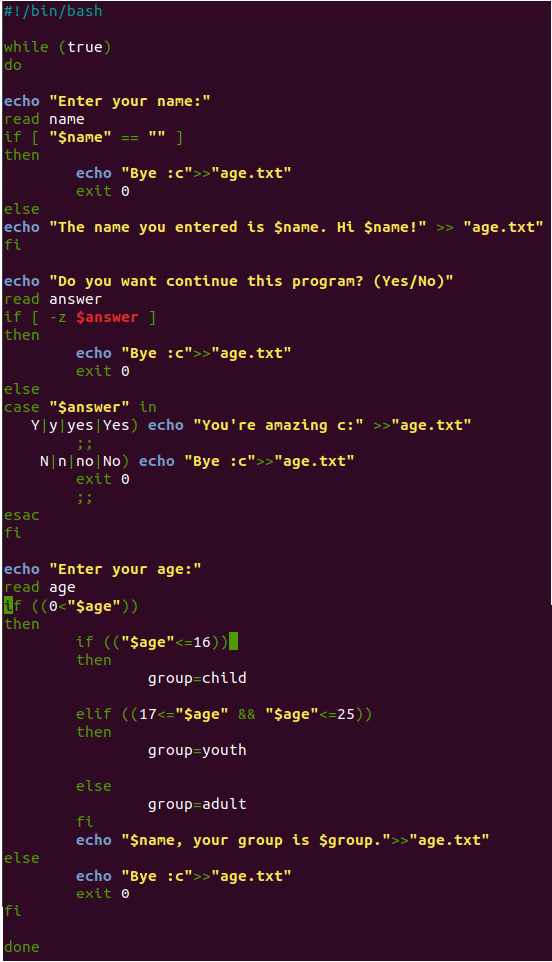
\includegraphics[width=0.7\textwidth]{script.png}
	\\
	\textit{Рисунок 2.1 скрипт для определения возрастной группы}	
	\\
\end{center}
	
\begin{center}
	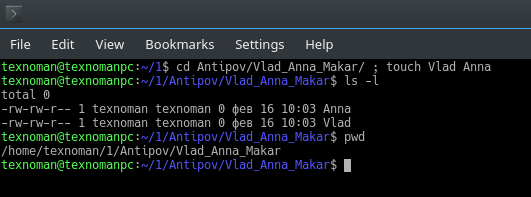
\includegraphics[width=0.7\textwidth]{4.png}
	\\
	\textit{Рисунок 2.2 Запуск, ход выполнения и завершение выполнения скрипта на терминале}
	\\	
\end{center}
	
\begin{center}
	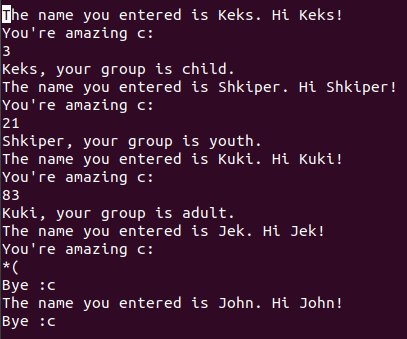
\includegraphics[width=0.7\textwidth]{5.png}
	\\
	\textit{Рисунок 2.3 текстовый файл age.txt с результатом работы скрипта}
	\\	
\end{center}
	

	
	